% Created 2018-11-28 Wed 21:38
% Intended LaTeX compiler: pdflatex
\documentclass[11pt]{article}
\usepackage[utf8]{inputenc}
\usepackage[T1]{fontenc}
\usepackage{graphicx}
\usepackage{grffile}
\usepackage{longtable}
\usepackage{wrapfig}
\usepackage{rotating}
\usepackage[normalem]{ulem}
\usepackage{amsmath}
\usepackage{textcomp}
\usepackage{amssymb}
\usepackage{capt-of}
\usepackage{hyperref}
\usepackage[margin=0.85in]{geometry}
\usepackage{booktabs}
\author{Cody Lewis}
\date{\today}
\title{Babyboom Data Analysis}
\hypersetup{
 pdfauthor={Cody Lewis},
 pdftitle={Babyboom Data Analysis},
 pdfkeywords={},
 pdfsubject={},
 pdfcreator={Emacs 26.1 (Org mode 9.1.9)},
 pdflang={English}}
\begin{document}

\maketitle
% latex table generated in R 3.5.1 by xtable 1.8-3 package
% Wed Nov 28 21:38:26 2018
\begin{table}[ht]
\centering
\begin{tabular}{rllll}
  \hline
 &      time &     sex &     weight &    minutes \\
  \hline
X & Min.   :   5.0   & female:18   & Min.   :1745   & Min.   :   5.0   \\
  X.1 & 1st Qu.: 792.8   & male  :26   & 1st Qu.:3142   & 1st Qu.: 482.8   \\
  X.2 & Median :1406.5   &  & Median :3404   & Median : 846.5   \\
  X.3 & Mean   :1296.0   &  & Mean   :3276   & Mean   : 788.7   \\
  X.4 & 3rd Qu.:1918.5   &  & 3rd Qu.:3572   & 3rd Qu.:1158.5   \\
  X.5 & Max.   :2355.0   &  & Max.   :4162   & Max.   :1435.0   \\
   \hline
\end{tabular}
\end{table}

\begin{center}
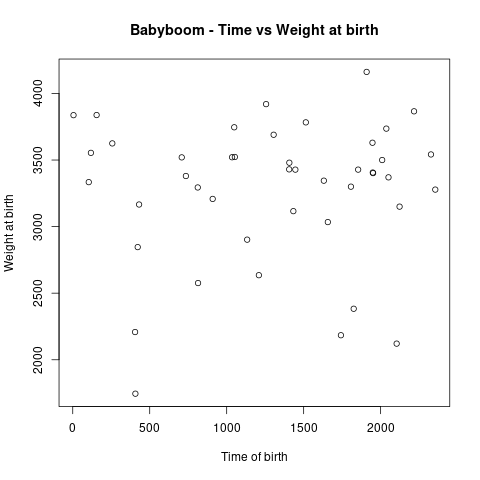
\includegraphics[width=.9\linewidth]{bb_time_weight.png}
\end{center}

\begin{center}
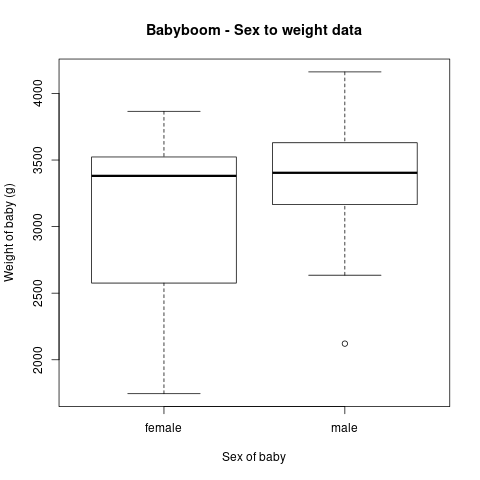
\includegraphics[width=.9\linewidth]{bb_weight_sex.png}
\end{center}

\begin{center}
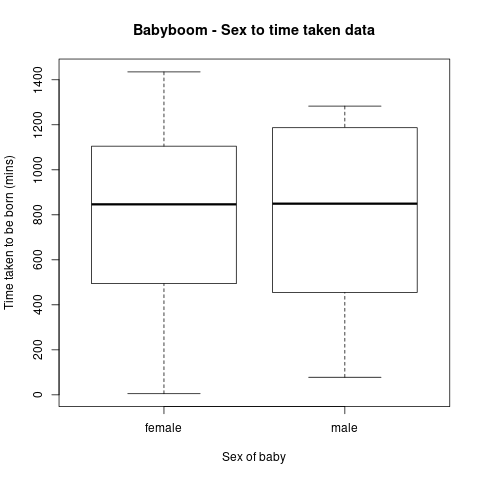
\includegraphics[width=.9\linewidth]{bb_minutes_sex.png}
\end{center}

\begin{center}
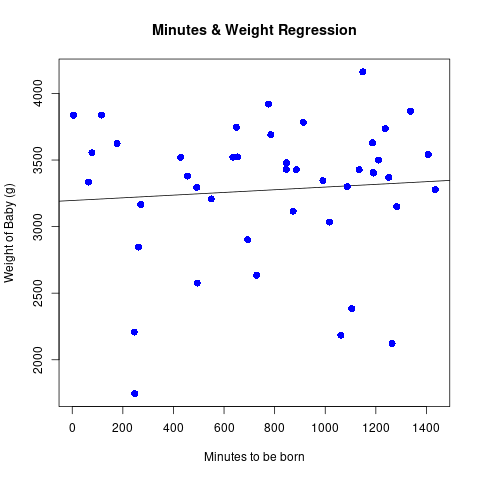
\includegraphics[width=.9\linewidth]{bb_minutes_weight.png}
\end{center}

% latex table generated in R 3.5.1 by xtable 1.8-3 package
% Wed Nov 28 21:38:27 2018
\begin{table}[ht]
\centering
\begin{tabular}{rrrrr}
  \hline
 & Estimate & Std. Error & t value & Pr($>$$|$t$|$) \\
  \hline
(Intercept) & 3196.2607 & 173.6416 & 18.41 & 0.0000 \\
  data\$minutes & 0.1010 & 0.1952 & 0.52 & 0.6074 \\
   \hline
\end{tabular}
\end{table}
\end{document}
